\section{功能需求}
    \subsection{CPU}
        CPU整体工作流程图
        \begin{figure}[!hbp]
                    \centering
                    \caption{CPU各阶段转换图}
                    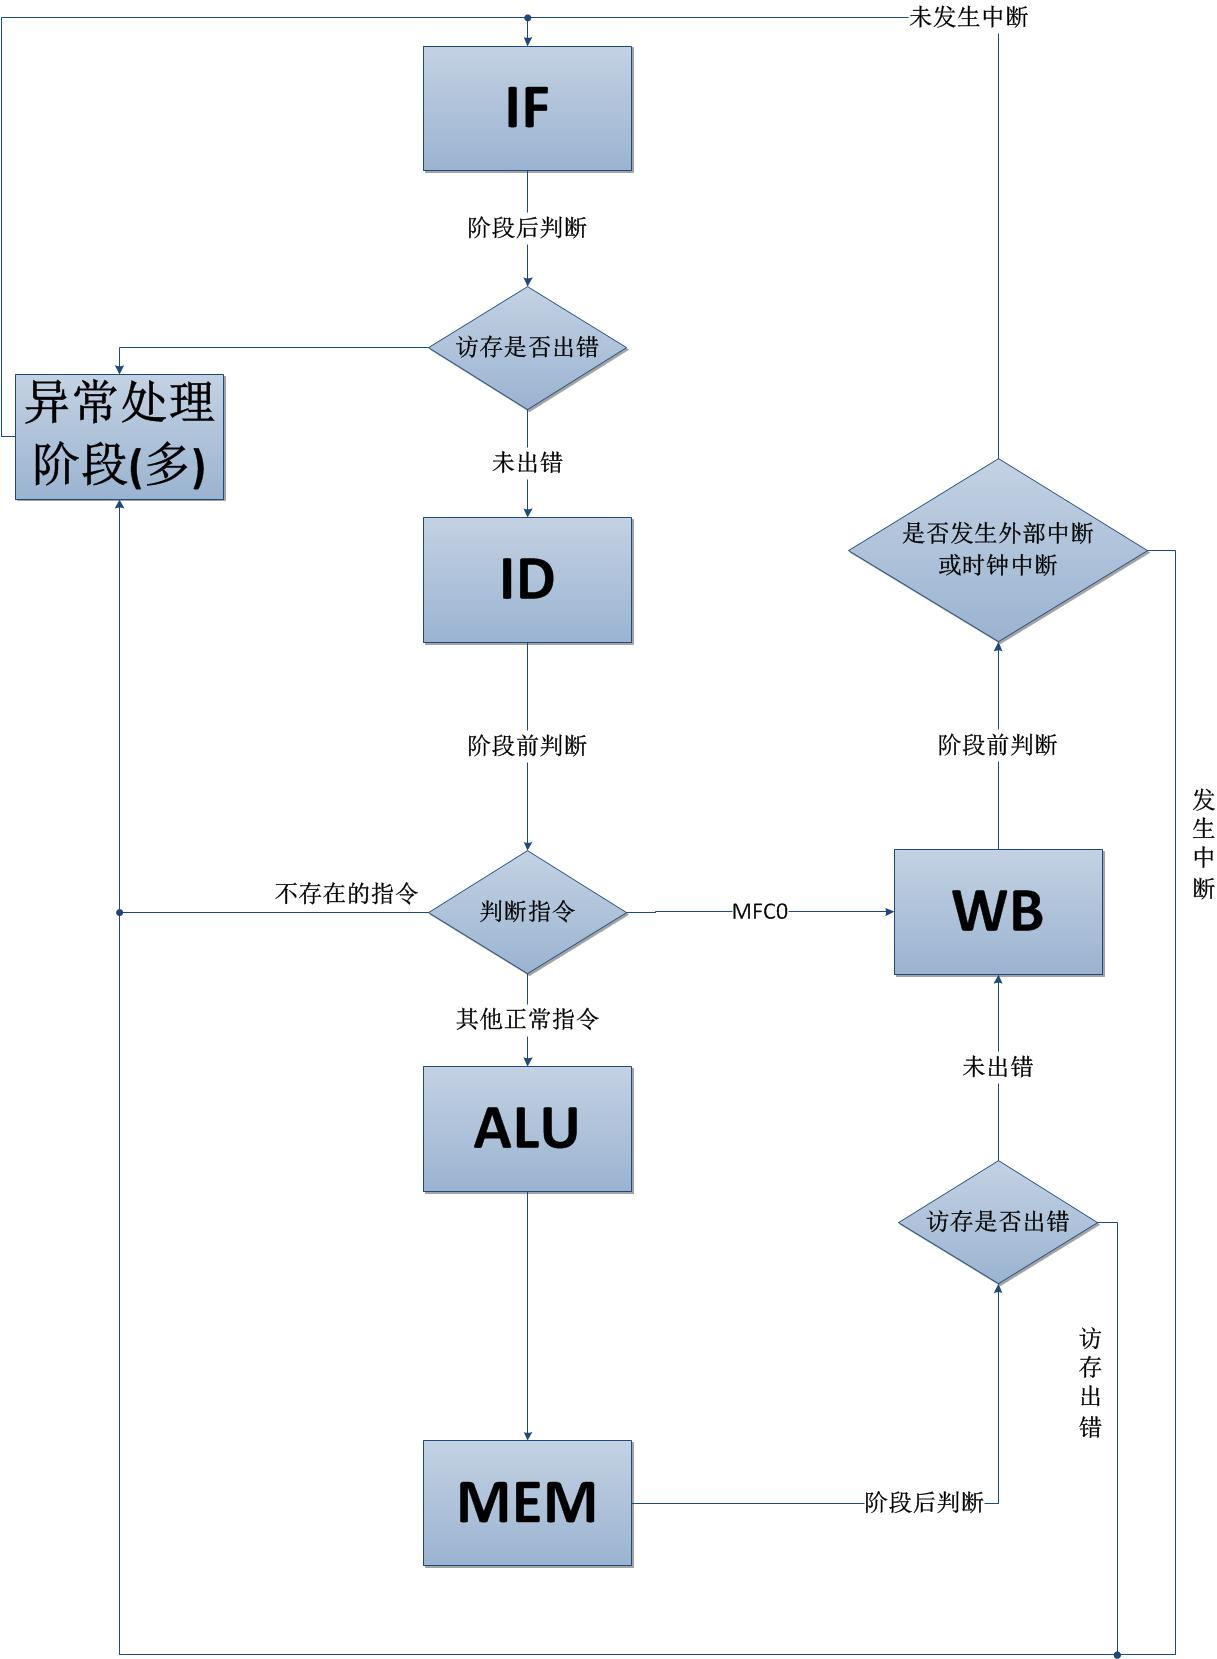
\includegraphics[width=0.75\textwidth]{picture/Stages.jpg}
        \end{figure}
                
        \subsubsection{ALU}
            功能需求:
            \begin{enumerate}
            \item
            完成数据和地址的算术、逻辑和移位运算,%
            输入两个数据根据ALUOp得出输出结果。
            \item
            根据指令系统的需求,完成指令系统中乘法之外的算术指令。
            \end{enumerate}

            实现方式:
            \begin{enumerate}
            \item
            ALU两个输入数据,ALUOp目前整理出9种运算。
            \item
            输出最终运算结果,三个标志位。
            \end{enumerate}

        \subsubsection{乘法器}
            功能需求:
            \begin{enumerate}
            \item
            完成乘法功能,结果保存在LO和HI寄存器中,可以访问计算结果。
            \end{enumerate}

            实现方式:
            \begin{enumerate}
                \item
            使用IPCore实现。
            \item
            是否与ALU放在一起,之后测试乘法器的速度再做决定。
            \item
            MFLO,MFHI,MTLO,MTHI,MULT指令查看。
            \end{enumerate}

        \subsubsection{CP0}
            功能需求:
            \begin{enumerate}
            \item
                辅助操作系统对硬件进行管理。
                \begin{enumerate}
                \item
                    内存管理:辅助操作系统,完成虚拟地址和物理地址的转换、不同进程之间的内存切换、用户态与内核态内存的分离
                \item
                    异常处理:检测指令执行过程中可能出现的异常、对异常进行分类、记录异常出现的指令地址或错误的内存地址
                \item
                    外部中断:负责检测外部中断,辅助实现CPU与外设之间的交互
                \end{enumerate}
            \item

            \end{enumerate}

            实现方式:
            具体实现方式参照下面两个小节。

            \begin{table}[!hbp]
            \centering
            \caption{需要实现的CP0寄存器}
            \begin{tabularx}{\textwidth}{|l|l|X|}
            \hline
            序号 & 名称 & 功能 \\
            \hline
            0 & Index & 用于TLBWI指令访问TLB入口的索引序号 \\
            \hline
            1 & EntryLo0 & 作为TLBWI及其他TLB指令接口,管理偶数页入口 \\
            \hline
            2 & EntryLo1 & 作为TLBWI及其他TLB指令接口,管理奇数页入口 \\
            \hline
            3 & EntryHi & TLB异常时,系统将虚拟地址部分写入EntryHi寄存器中用于TLB匹配 \\
            \hline
            4 & BadVAddr & 捕捉最近一次地址错误或TLB异常(重填、失效、修改)时的虚拟地址 \\
            \hline
            5 & Count & 每隔一个时钟周期增加1,用作计时器,并可使能控制 \\
            \hline
            6 & Compare & 当Count值与Compare相等时,SI\_TimerInt 引脚是变高电平直到有数值写入Compare,用于定时中断 \\
            \hline
            7 & Status & 表示协理器的操作模式、中断使能及诊断状态 \\
            \hline
            8 & Cause & 记录最近依次异常的原因,控制软件中断请求以及中断协理派分的向量 \\
            \hline
            9 & EPC & 存储异常处理之后程序恢复执行的地址 \\
            \hline
            10 & EBase & 识别多协理器系统中不同的协理器异常向量的基地址 \\
            \hline
            \end{tabularx}
            \end{table}

        \subsubsection{MMU与TLB}
            功能需求:
            \begin{enumerate}
            \item
                实现虚拟地址(线性地址)到物理地址的转换。% 
                只对部分地址% 
                ([0x20000000-0x80000000]和[0xC0000000-0xFFFFFFFF])% 
                进行地址映射,其余部分直接映射。
            \item
                实现内核态与用户态内存的区分。
            \item
                实现相对应的异常处理:TLBS、TLBL、TLB Modified。
            \end{enumerate}

            实现方式:
            \begin{enumerate}
            \item
                \begin{figure}[!hbp]
                    \centering
                    \caption{TLB电路结构}
                    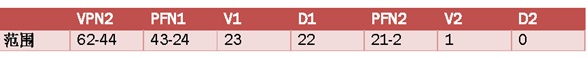
\includegraphics[width=0.9\textwidth]{picture/TLB.jpg}
                \end{figure}

                \begin{figure}[!hbp]
                    \centering
                    \caption{内存访问流程图}
                    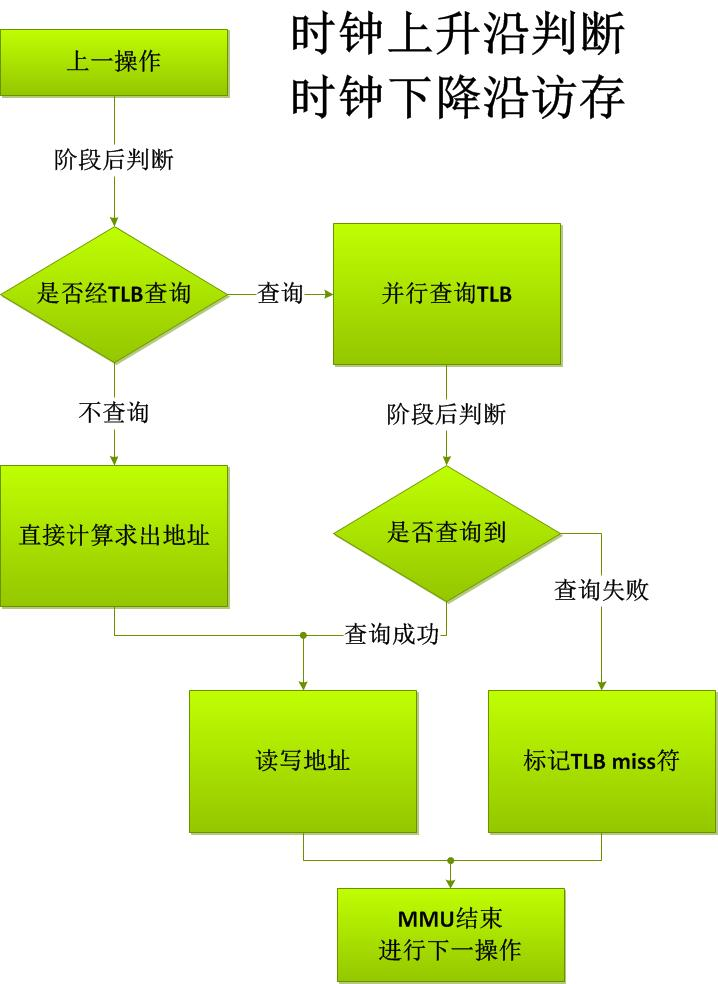
\includegraphics[width=0.75\textwidth]{picture/Memory.jpg}
                \end{figure}
                
                \begin{enumerate}
                \item
                    TLB共16项,每项可以将连续两个虚页映射到两个不同的物理页,相当于可以处理32个页
                \item
                    虚拟地址高19位作为虚页号VPN进行选择TLB表项,第20位通过奇偶判断,选择两个物理页之一
                \item
                    出于简化的考虑,不维护进程号ASID、全局标记G,默认所有G均为1,只维护每个物理地址的D标记
                \end{enumerate}

            \item
                硬件支持:
                \begin{enumerate}
                \item
                    虚拟地址高19位在TLB表项中并行查询EntryHi部分。
                \item
                    如果查找到,根据第20位选择EntryLo,直接与低12位结合得到真实的物理地址。
                \item
                    如果未查找到,触发TLBMiss异常:%
                    设置Cause寄存器中的ExcCode为TLB异常,%
                    EPC寄存器为当前指令的地址,%
                    BadvAddr寄存器为错误的地址,%
                    之后触发一个异常,PC跳转到EBase的异常处理基地址,%
                    之后由操作系统接管。
                \item
                    对于地址不对齐异常,在内存映射阶段对虚拟地址offset部分最低两位进行检测%
                    如果不为00,则触发地址不对齐异常,交由操作系统处理
                \end{enumerate}
            \item
                操作系统:
                \begin{enumerate}
                \item
                    进入异常处理向量(trap/vector.S)。
                \item
                    跳转到处理函数部分(trap/exception.S)。
                \item
                    先保存异常现场,之后进入mips\_trap函数(trap/trap.c)。
                \item
                    根据cause寄存器的值进行分类,调用handle\_tlbmiss函数。
                \item
                    得到异常地址对应的物理页号,%
                    之后进行tlb\_refill(include/thumips\_tlb.h)。
                \item
                    操作系统维护index,%
                    写EntryLo0、EntryLo1、EntryHi、 PageMask、Index五个寄存器,%
                    之后用tlbwi写到TLB的第Index项。%
                    此处需要硬件提供MTC0、MFC0、TLBWI指令的支持。
                \item
                    异常返回,重新执行取地址命令。%
                \end{enumerate}
            \end{enumerate}

        \subsubsection{异常中断处理}
            功能需求:
            \begin{enumerate}
            \item
            实现对异常和外部中断的处理。
            \item
            实现的异常有内存访问异常、地址不对齐异常、%
            系统调用、未定义的指令异常、未定义的寄存器异常。
            \item
            外部中断:键盘、通讯端口。
            \end{enumerate}

            实现方式:
            \begin{figure}[!hbp]
                    \centering
                    \caption{异常中断处理流程}
                    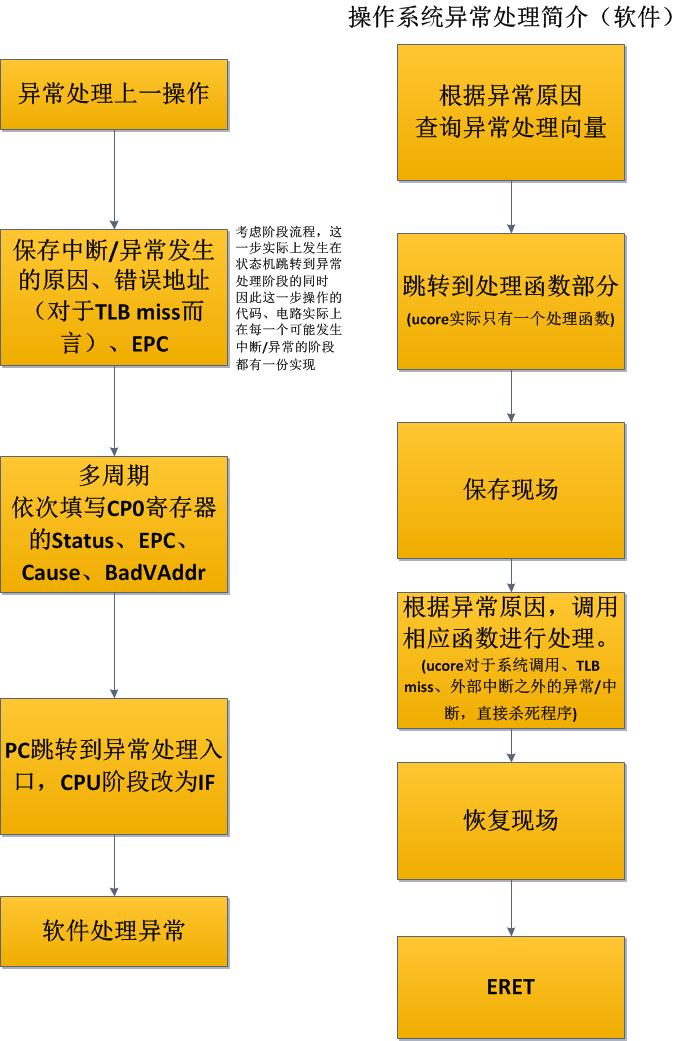
\includegraphics[width=0.9\textwidth]{picture/Exception.jpg}
            \end{figure}
                
            \begin{table}
            \centering
            \caption{需要实现的异常}
            \begin{tabular}{|c|c|c|}
            \hline
            异常号 & 异常名 & 描述 \\
            \hline
            0 & Interrupt & 外部中断,异步发生,由硬件引起 \\
            \hline
            1 & TLB Modified & 内存修改异常, 发生在Memory阶段 \\
            \hline
            2 & TLBL & 读未在TLB中映射的内存地址触发的异常 \\
            \hline
            3 & TLBS & 写未在TLB中映射的内存地址触发的异常 \\
            \hline
            4 & ADEL & 读访问一个非对齐地址触发的异常 \\
            \hline
            5 & ADES & 写访问一个非对齐地址触发的异常 \\
            \hline
            8 & SYSCALL & 系统调用 \\
            \hline
            10 & RI & 执行未定义指令异常 \\
            \hline
            11 & Co-Processor Unavailable & 试图访问不存在的协处理器异常 \\
            \hline
            \end{tabular}
            \end{table}

            \begin{enumerate}
            \item
            硬件支持
                \begin{enumerate}
                \item
                异常处理,在数据通路上添加异常处理部分,%
                在多周期的任意一个周期检测到异常后,%
                在Cause设置异常代码、
                在EPC寄存器设置异常处理的返回地址,
                将Status寄存器的EXL为设置为1,表示进入内核态处理异常
                之后根据EBase跳转到异常处理向量基地址,%
                之后操作系统接管。
                \item
                外部中断处理,设置外部中断检查信号,外部设备触发时,%
                异步地将检查信号置1;每个指令IF阶段检查该信号,%
                若为1则进入外部中断处理,否则正常执行指令。
                \item
                时钟中断处理。当寄存器Count和Compare寄存器中的数值相等时,%
                触发一个时钟异常,交由操作系统处理。
                \end{enumerate}
            \item
            操作系统
                \begin{enumerate}
                \item
                进入异常处理向量(trap/vector.S)。
                \item
                跳转到处理函数部分(trap/exception.S)。
                \item
                先保存异常现场,之后进入mips\_trap函数(trap/trap.c)。
                \item
                根据cause寄存器的值进行分类,%
                调用interrupt\_handler、syscall等等函数进行处理,%
                如果是地址不对齐异常,未定义的指令或未定义的异常,直接退出。
                \item
                使用ERET指令从异常返回,将EXL位重新设置为0,表示进入用户态
                重新执行取地址命令
                \end{enumerate}
            \end{enumerate}

        \subsubsection{其他功能部件}
            \paragraph{PC}
                \mbox{} \\ 

                功能需求:
                \begin{enumerate}
                \item
                实现PC的多种变换方式:正常执行、分支、跳转。
                \item
                实现异常处理时对PC的处理,跳转到异常处理向量部分。
                \end{enumerate}

                实现方式
                \begin{enumerate}
                \item
                通过多路选择器选择ALU的输入数据,与当前PC进行运算%
                实现PC的多种变化方式。
                \end{enumerate}

            \paragraph{寄存器堆}
                \mbox{} \\ 

                功能需求:
                \begin{enumerate}
                \item
                实现通用寄存器,以及在数据通路中的读写控制。
                \end{enumerate}

                实现方式
                \begin{enumerate}
                \item
                在CPU中实现寄存器堆并实现读写控制。
                \end{enumerate}

            \paragraph{串口}
                \mbox{} \\

                功能需求:
                \begin{enumerate}
                \item
                实现与PC机通信,通过计算机键盘输入数据,向计算机输出数据。
                \end{enumerate}

                实现方式
                \begin{enumerate}
                \item
                使用开源的%
                \href{http://www.fpga4fun.com/SerialInterface.html}{ASync transmitter and receiver},%
                通过在每个信号周期内多次采样,并滤波得到稳定的信号。%
                CPLD仅负责TX/RX端口数据的转发,%
                对数据的编码与解码在FPGA中进行。%
                这样设计提高了数据传送的准确率,%
                并且串口数据不需要占用内存数据线,%
                无需处理冲突,简化了设计。%
                数据通信协议在开发过程中设计,有待进一步说明。

                \end{enumerate}
        \subsubsection{扩展部分}
            目前没有关于扩展部分的想法,先完成基本部分。

            网络部分比较有明确的开发目标,但组内无操作系统开发经验。

            测试工具部分没有明确的开发目标,不太清楚如何入手开发。

        \subsubsection{指令集与数据通路}
            指令集为标准MIPS系统子集

            实现多周期CPU,针对指令集设计数据通路。
            仿照《软件硬件接口》书中的多周期CPU进行设计,
            在书中7条指令的原型上进行扩展,以支持标准MIPS系统的子集。
            
            指令执行过程主要分为取指、解码、执行、访存、写回五个周期,
            某些指令可能需要其他特殊的周期支持,采用多周期实现比较灵活。

            数据通路包括状态机与控制线设计,每条指令有不同的状态机变化,
            而且对指令进行解码,能够得到相应的控制线。%
            在多周期的不同周期利用控制线对数据通路进行控制,使指令正常执行。
            
            \begin{figure}[!hbp]
                    \centering
                    \caption{数据通路设计图}
                    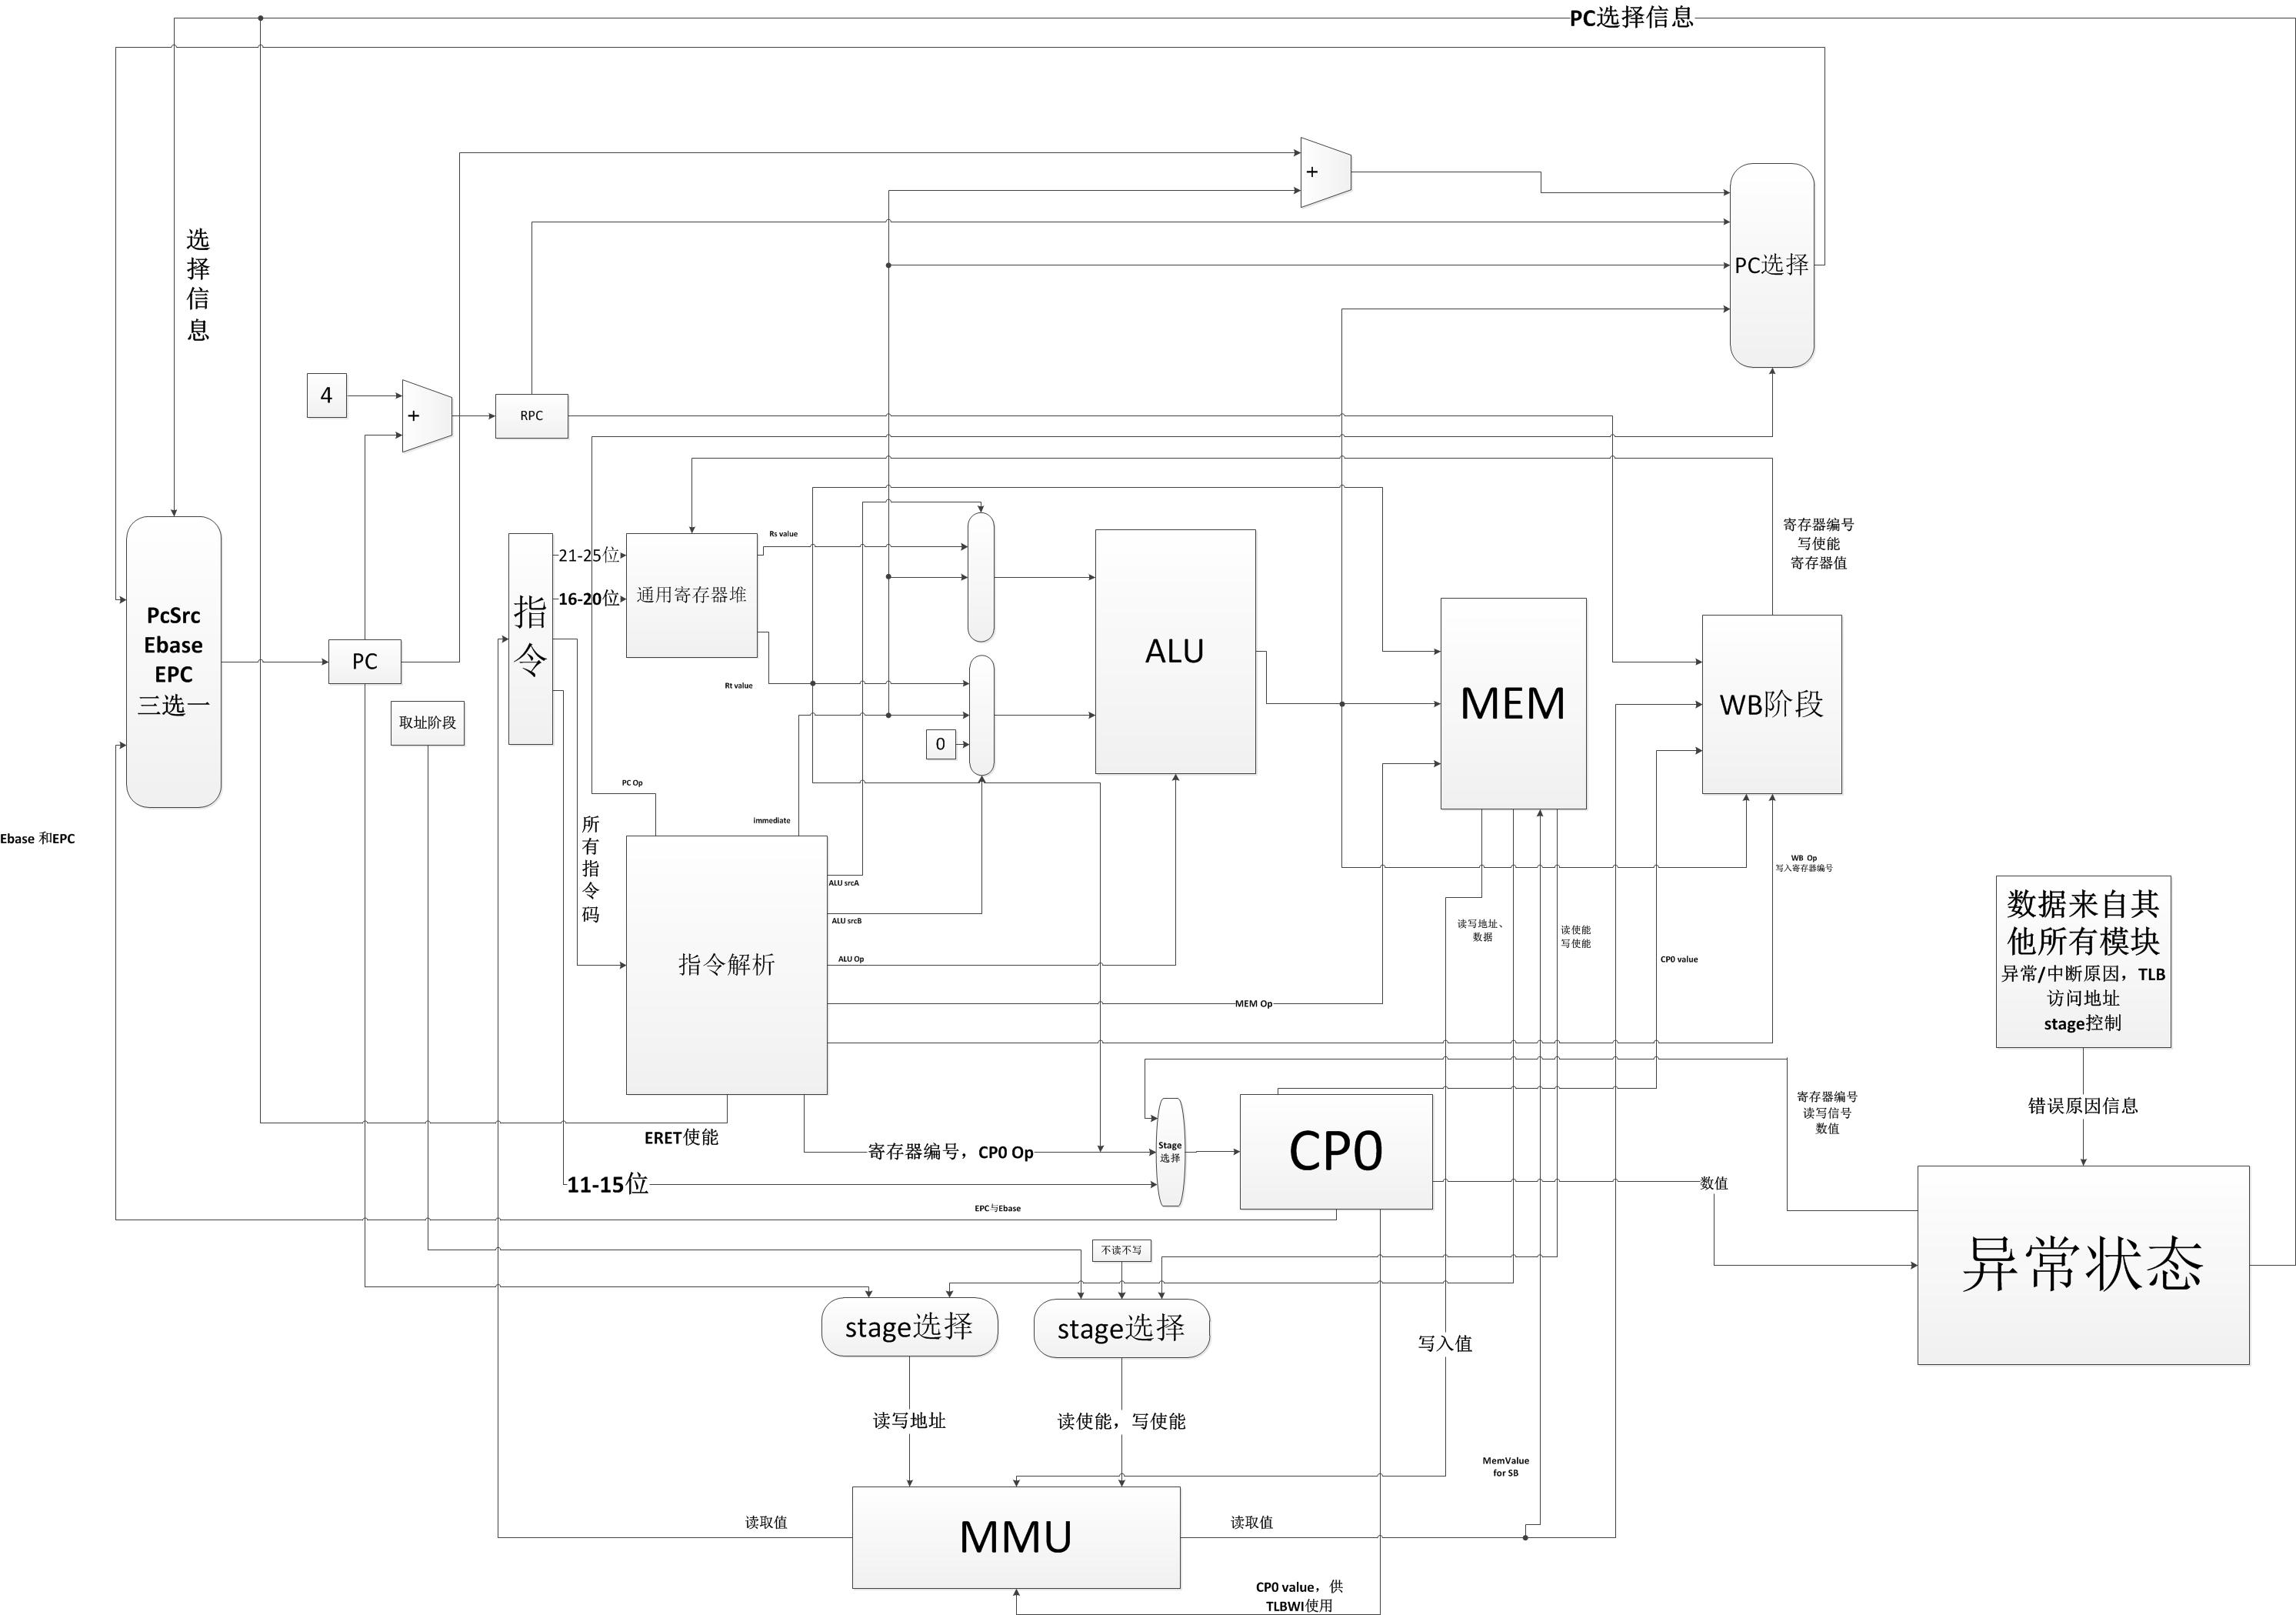
\includegraphics[width=\textwidth]{picture/CPU_Design.jpg}
            \end{figure}

    \subsection{BIOS}
        准备阶段:操作系统和其他程序烧写到Flash中,%
        bootasm.S编译出的二进制文件写到ROM中,再把CPU写到FPGA中。

        启动阶段:从ROM中的bootasm.S启动,%
        将Flash中的全部操作系统拷贝到RAM中,然后控制权交给操作系统。

        操作系统启动:bootasm.S工作结束后,进入操作系统entry.S文件中进行寄存器初始化。
        包括对通用寄存器,CP0寄存器,异常处理基地址进行初始化,之后跳转到init.c中的kern\_init。
        在此完成TLB初始化,中断异常的初始化,物理内存与虚拟内存的转换页表的初始化,
        最后完成操作系统的进程和文件管理系统,至此ucore系统开始正常工作



